% =====================================================================
%  Data Engineering (34623) - Semester Project
%  Checkpoint 2: Architecture, ETL & Monitoring - Written Status Update
%  Universidad San Jorge - Lecturer: Luis Palazón Simón
%  Compile with: latexmk -pdf checkpoint2_status_update.tex
% =====================================================================
\documentclass[11pt,a4paper]{article}

% ---------- Packages ----------
\usepackage[utf8]{inputenc}
\usepackage[T1]{fontenc}
\usepackage[english]{babel}
\usepackage{lmodern}
\usepackage[margin=2.3cm]{geometry}
\usepackage{booktabs}
\usepackage{tabularx}
\usepackage{enumitem}
\usepackage{xcolor}
\usepackage{tikz}
\usetikzlibrary{positioning,arrows.meta}
\usepackage{hyperref}
\hypersetup{colorlinks=true, linkcolor=blue!50!black, urlcolor=blue!50!black}

% ---------- Helper macros ----------
\newcolumntype{Y}{>{\raggedright\arraybackslash}X}
\setlist{nosep, leftmargin=*}

% ---------- Project metadata ----------
\newcommand{\projecttitle}{TETR.IO Player Progression Analytics}
\newcommand{\teamname}{Hueskers}
\newcommand{\submissiondate}{25/11/2026}
\newcommand{\repourl}{\url{https://github.com/inaTrip/tetrio-analytics}}

% =====================================================================
\begin{document}

\begin{center}
  {\Large\bfseries Data Engineering -- Semester Project}\\[4pt]
  {\large Checkpoint 2: Architecture, ETL \& Monitoring}\\[8pt]
  {\large\itshape \projecttitle}\\[8pt]
  Team: \teamname \quad$\cdot$\quad Date: \submissiondate\\
  Repository: \repourl
\end{center}
\vspace{2mm}\hrule\vspace{4mm}

% =====================================================================
\section{Progress Summary}
\begin{tabularx}{\textwidth}{@{}p{4.6cm}p{2.6cm}Y@{}}
\toprule
\textbf{Checkpoint 2 item} & \textbf{Status} & \textbf{Evidence in the repository} \\
\midrule
Lifecycle mapping & Done & \texttt{docs/architecture.md} (Section~\ref{sec:lifecycle}) \\
Architecture / cluster design & Done & \texttt{docs/architecture.md} (Section~\ref{sec:arch}) \\
Working ingestion \& integration & Working & \texttt{src/ingestion/}, \texttt{src/transformation/}, \texttt{src/quality/} \\
Data warehouse model & Built and loaded & \texttt{warehouse/schema.sql}, \texttt{warehouse/load.sql} \\
Orchestration plan & Interim schedule running & \texttt{orchestration/crontab.txt}, \texttt{docs/orchestration.md} \\
Logging \& alerting design & Logging implemented; alerting designed & \texttt{src/monitoring/logger.py}, \texttt{docs/monitoring.md} \\
\bottomrule
\end{tabularx}

\medskip
\noindent\textbf{Changes since Checkpoint 1.} The team continues with two
datasets (D1: TETR.IO API, daily; D2: Kaggle Tetra League snapshot,
September 2023), which meets the 2--5 requirement and keeps a clean
player-level join. The overlap between both sources, announced in
Checkpoint 1 as ``to be measured in the first full ingestion run'', has now
been measured on the complete leaderboard (Section~\ref{sec:results}).

% =====================================================================
\section{Lifecycle Mapping}\label{sec:lifecycle}
The pipeline follows an ETL pattern with a raw landing layer: raw data is
stored unchanged before it is transformed, so any day can be reprocessed.
\begin{center}
\small
\begin{tabularx}{\textwidth}{@{}p{2.6cm}Y@{}}
\toprule
\textbf{Stage} & \textbf{Process in this project} \\
\midrule
Generation & TETR.IO servers produce player statistics; Kaggle author produced the 2023 baseline. \\
Ingestion & Paginated, rate-limited API download (daily); one-off Kaggle download; data minimisation. \\
Storage & Raw JSON per day, curated Parquet, DuckDB star schema. \\
Processing & Flattening, common schema, sentinels to null, quality checks, 2023 $\leftrightarrow$ today join, SCD type 2, load. \\
Analysis & SQL queries on the star schema, daily sanity check; dashboard planned. \\
Archival / Deletion & Raw kept, compressed and moved to cold storage after 90 days; logs kept 30 days. A player is deleted by removing them from the raw files: the full refresh removes them downstream. Defined, not yet automated. \\
\bottomrule
\end{tabularx}
\end{center}
Details: \texttt{docs/architecture.md}.

% =====================================================================
\section{Architecture and Cluster Design}\label{sec:arch}
\begin{itemize}
  \item \textbf{Single node:} about 99\% of each run ($\sim$450\,s) is spent
        waiting between API requests, which the API rules limit to about one
        per second; processing and loading $\sim$117{,}000 rows takes about
        2\,s. More machines would add cost without making ingestion faster.
  \item \textbf{When a single node stops being enough:} daily full refresh of
        a growing history (incremental loads), $\times 10$ rows (ingestion
        above one hour: parallel requests if allowed), $\times 1{,}000$ and
        beyond (data no longer fits one machine: serverless cloud warehouse or
        distributed processing). Preferred path: scale up, then serverless,
        rather than operating our own cluster.
  \item \textbf{Warehouse:} DuckDB now (free, no server, columnar); BigQuery
        for the cloud version (Python SDK, Looker Studio). PostgreSQL was
        discarded: row-based storage suits transactions better than analytics.
  \item \textbf{Environmental impact:} daily batch only, no always-on
        infrastructure; the main long-term cost is raw storage
        ($\sim$4.2\,GB/year), reduced by compression and cold storage.
\end{itemize}

% =====================================================================
\section{Working Ingestion and Integration}\label{sec:ingestion}
The complete pipeline runs end to end with one command
(\texttt{python -m src.pipeline}) on real data:

\begin{itemize}
  \item \textbf{Ingestion D1} (\texttt{tetrio\_api.py}): fetches the complete
        Tetra League leaderboard page by page (100 players per page), paced at
        one request per second as required by the API rules, with an
        identifying \texttt{User-Agent}, one \texttt{X-Session-ID} per run, and
        up to 5 retries with increasing waits on HTTP~429/5xx and network
        errors. The raw response is saved as one JSON file per day; the file is
        written to a temporary name and then renamed, so a failed run never
        leaves a half-written file.
  \item \textbf{Data minimisation:} only the player ID, username, country and
        league statistics are stored; other profile fields (e.g.\ biography,
        linked social accounts) are discarded before reaching disk.
  \item \textbf{Ingestion D2} (\texttt{kaggle\_loader.py}): one-off download
        through the \texttt{kaggle} CLI, skipped if the file already exists.
  \item \textbf{Processing} (\texttt{transform.py}): both sources are mapped
        to one common schema: the nested \texttt{league} object is flattened,
        \texttt{\_id}/\texttt{id} become \texttt{player\_id}, negative sentinel
        values (e.g.\ \texttt{-1} for hidden counts) become null, types are
        made explicit (nullable integers and floats), ranks are lower-cased and
        country codes upper-cased.
  \item \textbf{Quality checks} (\texttt{checks.py}): rows without ID,
        duplicated player/date pairs and TR values outside 0--25{,}000 are
        removed, and every rule logs how many rows it rejected.
  \item \textbf{Integration} (\texttt{integrate.py}): the curated layer
        (Parquet) is rebuilt from all raw files on every run, which makes the
        step idempotent (re-running never creates duplicates). It produces the
        snapshot table, a player table and the 2023~$\leftrightarrow$~today
        progression join on \texttt{player\_id}.
  \item \textbf{Tests:} 5 unit tests (\texttt{pytest}) cover the schema
        mapping, the sentinel conversion, the quality rules, the SCD type~2
        logic and the rank order.
\end{itemize}

% =====================================================================
\section{First Full Run: Results}\label{sec:results}
\begin{tabularx}{\textwidth}{@{}p{6.4cm}Y@{}}
\toprule
\textbf{Measure (first manual run, 22/11/2026)} & \textbf{Value} \\
\midrule
Players fetched / pages / duration & 36{,}094 / 361 / 420\,s \\
Duplicates removed by quality checks & 2 (players moving between pages during pagination) \\
Ranked players: 2023 vs.\ 2026 & 45{,}197 vs.\ 36{,}092 ($-20\%$) \\
Current players already ranked in 2023 & 6{,}188 of 36{,}092 (17\%) \\
Fact rows = staged rows (integrity check) & 81{,}289 = 81{,}289 \\
Players with a changed username or country & 687 (75{,}788 versions for 75{,}101 players) \\
Daily snapshots collected so far & 3 (22, 23 and 24/11), one per scheduled run \\
\bottomrule
\end{tabularx}

\medskip
\noindent The 17\% overlap on the full leaderboard is much lower than the
62\% measured on the top 500 players in Checkpoint~1: long-term players are
concentrated at the top of the leaderboard.

\medskip
\noindent\textbf{Scheduled runs.} The scheduled runs fetched 36{,}059
(22/11), 35{,}994 (23/11) and 36{,}014 (24/11) players, in 450--460\,s each,
with the integrity check passing every time. The scheduled run of 22/11
replaced the snapshot of that day's manual run, as designed: there is one
snapshot per day, and a re-run on the same day overwrites it.

\paragraph{First insight: what changes with rank.} Average values in the
latest snapshot. Attack per piece $=$ APM\,/\,(PPS\,$\times$\,60).

\begin{center}
\small
\begin{tabular}{@{}lrrrrrrrrr@{}}
\toprule
Rank & d & c & b & a & s & ss & u & x & x+ \\
\midrule
APM             & 6.7  & 12.8 & 19.3 & 28.6 & 46.7 & 72.5 & 98.7 & 139.4 & 182.4 \\
PPS             & 0.71 & 0.88 & 1.07 & 1.27 & 1.60 & 1.97 & 2.36 & 2.92  & 3.49  \\
Attack per piece & 0.16 & 0.24 & 0.30 & 0.38 & 0.49 & 0.61 & 0.70 & 0.80  & 0.87  \\
\bottomrule
\end{tabular}
\end{center}

\noindent From rank d to x+, speed (PPS) grows about $\times 5$ and efficiency
(attack per piece) about $\times 5.5$; together they explain the $\times 27$
increase in APM. Because ranks are percentile-based, the $-20\%$ drop
appears in every tier and reflects fewer ranked players overall, not a change
in skill.

% =====================================================================
\section{Data Warehouse Model}\label{sec:dw}
\begin{center}
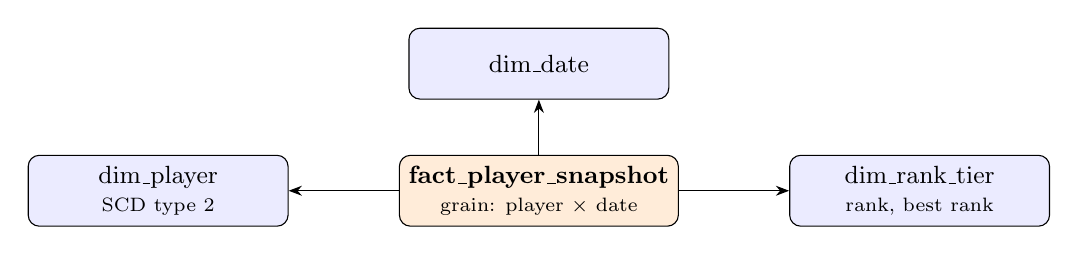
\begin{tikzpicture}[
  tbl/.style={draw, rounded corners, align=center, font=\small,
              minimum width=3.3cm, minimum height=0.9cm},
  >=Stealth]
  \node[tbl, fill=orange!15] (f) {\textbf{fact\_player\_snapshot}\\[-1pt]
        {\scriptsize grain: player $\times$ date}};
  \node[tbl, fill=blue!8, left=1.4cm of f]  (p) {dim\_player\\[-1pt]{\scriptsize SCD type 2}};
  \node[tbl, fill=blue!8, right=1.4cm of f] (r) {dim\_rank\_tier\\[-1pt]{\scriptsize rank, best rank}};
  \node[tbl, fill=blue!8, above=0.7cm of f] (d) {dim\_date};
  \draw[->] (f) -- (p);
  \draw[->] (f) -- (r);
  \draw[->] (f) -- (d);
\end{tikzpicture}
\end{center}

\begin{itemize}
  \item \textbf{Engine:} DuckDB, a local file-based analytical (columnar)
        database: free, no server, reads Parquet directly. The SQL is kept in
        separate files to be ported to a cloud warehouse (BigQuery) later.
  \item \textbf{Fact table:} TR, Glicko, RD, GXE, APM, PPS, VS, games played
        and won, decaying flag; \texttt{source} is kept as a degenerate
        dimension.
  \item \textbf{SCD type 2 player dimension:} a change of username or country
        creates a new version with its own validity period, so history is
        kept instead of overwritten (687 players on real data).
  \item \textbf{Point-in-time join:} each fact row is linked to the player
        version valid on its date, so a 2023 row shows the 2023 username.
  \item \textbf{Rank dimension:} ranks are taken from the source with an
        explicit order (d $<$ \dots $<$ x+); unknown codes are added instead
        of failing the load (the new rank x+ and the unranked code z already
        appear in the data).
  \item \textbf{Load:} full refresh inside one transaction; if the
        integrity check fails (staged rows $\neq$ fact rows), the previous
        warehouse is kept unchanged.
\end{itemize}

% =====================================================================
\section{Orchestration Plan}\label{sec:orch}
The API keeps no history, so a missed day can never be recovered: the
pipeline must run daily.

\begin{itemize}
  \item \textbf{Now (interim):} a cron job runs the pipeline every day at
        21:07 on a team member's machine (\texttt{orchestration/crontab.txt}).
        It was set up first so that daily snapshots started being collected
        immediately. Limitation: it only runs while that machine is on.
  \item \textbf{Target:} a scheduled GitHub Actions workflow writing to cloud
        storage (Google Cloud Storage + BigQuery). The runner is temporary,
        so persistent cloud storage is a precondition of this migration.
  \item \textbf{Alternatives considered:} Apache Airflow (overkill for one
        daily job, always-on infrastructure) and GCP Cloud Scheduler with
        Cloud Run (good fit, but more setup and stronger lock-in).
  \item \textbf{Safe to schedule:} idempotent steps, atomic writes,
        transactional load, exit code 0/1 for success/failure.
\end{itemize}
Full comparison and migration steps: \texttt{docs/orchestration.md}.

% =====================================================================
\section{Logging and Alerting Design}\label{sec:monitoring}
\textbf{Logging (implemented).} Every module logs through one shared logger
to the console and to \texttt{logs/pipeline.log}, with timestamp, level and
module. Each stage logs its key figures: pages and players fetched, retries,
rows in/out of each quality rule, overlap of the join, rows loaded per table,
and the full traceback of any failure.

\medskip
\noindent\textbf{Alerting (design).} Thresholds are based on the runs
observed so far ($\sim$0.2\% daily change in player count, $\sim$450\,s per
run).
\begin{center}
\small
\begin{tabularx}{\textwidth}{@{}Yp{2.3cm}p{2.6cm}@{}}
\toprule
\textbf{Condition} & \textbf{Severity} & \textbf{Threshold} \\
\midrule
Pipeline failed (includes 0 players fetched and a failed integrity check) & Critical & Any failure \\
Player count changed vs.\ the previous day & Warning / Critical & $>5\%$ / $>20\%$ \\
Rows rejected by quality checks & Warning & $>1\%$ \\
Run much slower than usual & Warning & $>900$\,s \\
Many API retries in one run & Warning & $>10$ \\
No new snapshot (the scheduler did not run) & Critical & $>26$\,h \\
\bottomrule
\end{tabularx}
\end{center}
\begin{itemize}
  \item \textbf{Silent failures:} if the scheduler does not run, the pipeline
        cannot alert about itself, so the last condition needs an independent
        heartbeat check outside the pipeline.
  \item \textbf{Channel:} a Discord webhook to a team channel (URL kept as a
        secret, never committed), plus GitHub's built-in failure e-mail once
        the pipeline runs on GitHub Actions.
  \item \textbf{Alert fatigue:} one message per run listing every triggered
        condition; no message on normal runs; retries handled automatically
        are not alerts; thresholds reviewed after the first weeks of data.
  \item \textbf{Implementation (planned before the presentation):}
        \texttt{src/monitoring/alerts.py}, called from the \texttt{except}
        block of \texttt{src/pipeline.py} and after each successful run.
\end{itemize}
Details: \texttt{docs/monitoring.md}.

% =====================================================================
\section{Risks and Next Steps}
\begin{itemize}
  \item \textbf{Single machine:} until the GitHub Actions migration, a day is
        lost whenever the scheduling machine is off.
  \item \textbf{Rank comparability:} the rank ladder changed (x+ added), so
        rank changes between 2023 and 2026 are interpreted with care.
  \item \textbf{Next steps:} cloud storage and BigQuery via the Python SDK;
        GitHub Actions schedule; alerting implementation; dashboard (Looker
        Studio); scalability analysis and cloud migration cost estimate.
\end{itemize}

% =====================================================================
\section{Work Organisation}\label{sec:kanban}
The team adopted a Kanban board on 23/11/2026 (GitHub Projects, linked to the
repository).

\begin{itemize}
  \item \textbf{Board columns:} Backlog $\rightarrow$ Ready $\rightarrow$
        In progress $\rightarrow$ In review $\rightarrow$ Done. Cards move
        automatically to Done when the linked pull request is merged.
  \item \textbf{One issue per task}, each with an owner, a milestone and a
        checklist that defines when it is done.
  \item \textbf{Milestones:} Checkpoint 2 (25/11), Oral presentation (21/12),
        Final delivery (10/01/2027). The remaining work is already in the
        backlog: cloud storage and BigQuery, GitHub Actions, alerting
        implementation, dashboard, scalability and cost analysis, data
        consumers, privacy and AI reflections.
  \item \textbf{Workflow:} each task is developed in its own branch and
        merged through a pull request that references its issue
        (\texttt{Closes \#N}); no direct commits to \texttt{main}.
  \item \textbf{WIP limit:} at most two cards in progress per person, to
        finish work before starting new work.
  \item \textbf{Before the board:} work up to 22/11 was tracked through pull
        requests (\#1--\#10); these were added to the board as Done items.
\end{itemize}

% =====================================================================
\section*{AI Usage Disclosure}
In line with Section~8 of the project kickoff document, this section states
which parts of the work presented at this checkpoint were generated or
assisted by AI. The full record, including the prompt used for each
component, is kept in \texttt{docs/ai\_usage\_disclosure.md}.

\paragraph{Tool and model.} Claude (Anthropic), model Claude Opus 5.5,
used through the Claude desktop application in November 2026.

\paragraph{Generated components.}
\begingroup\raggedright
\begin{itemize}
  \item \textbf{Pipeline code} (\texttt{src/settings.py},
        \texttt{src/pipeline.py}, \texttt{src/ingestion/},
        \texttt{src/transformation/}, \texttt{src/quality/},
        \texttt{src/monitoring/logger.py}, \texttt{tests/test\_transform.py}).
  \item \textbf{Warehouse} (\texttt{warehouse/*.sql},
        \texttt{src/load/warehouse.py}, \texttt{tests/test\_warehouse.py},
        \texttt{notebooks/explore\_warehouse.py}).
  \item \textbf{Cron configuration} (\texttt{orchestration/crontab.txt}).
  \item \textbf{Daily sanity check} (\texttt{notebooks/check\_daily.py}).
  \item \textbf{Documentation} (\texttt{docs/orchestration.md},
        \texttt{docs/architecture.md}, \texttt{docs/monitoring.md}).
  \item \textbf{This document} (structure, wording and the summaries of the
        documents above).
\end{itemize}
\endgroup

\paragraph{Team contribution.} The team ran every component on real data,
checked and shared the outputs, which revealed errors that were then
corrected (e.g.\ a grouping error in an example query), and chose the theme,
the datasets and the schedule. The generated code was used without manual
changes; the documents were reviewed and edited by the team.

\paragraph{Responsibility.}
All AI output was reviewed by the team. The team is responsible for the
final content and can explain and defend every part of it.

\end{document}
